% ======================================================================
% Magnetic cilia tactile skin — Nature Sensors target manuscript
% Master file. Compile: pdflatex -> bibtex -> pdflatex x2
% All missing numbers are marked [DATA NEEDED: ...]. No data are invented.
% ======================================================================
\documentclass[11pt]{article}

\usepackage[a4paper,margin=2.5cm]{geometry}
\usepackage[utf8]{inputenc}
\usepackage[T1]{fontenc}
\usepackage{amsmath,amssymb}
\usepackage{graphicx}
\usepackage{xcolor}
\usepackage{lineno}
\usepackage[numbers,super,sort&compress]{natbib}
\usepackage{setspace}
\usepackage{caption}
\usepackage[colorlinks=true,linkcolor=blue,citecolor=blue,urlcolor=blue]{hyperref}

% ---- placeholder command: every missing number MUST use this ----------
\newcommand{\dataneeded}[1]{\textcolor{red}{[DATA NEEDED: #1]}}
% ---- reference placeholder: never fabricate citations -----------------
\newcommand{\refneeded}[1]{\textcolor{orange}{[REF NEEDED: #1]}}

\captionsetup{font=small,labelfont=bf}
\graphicspath{{figures/}}

\title{\textbf{A full-hand magnetic cilia tactile skin for spatially
distributed perception of subtle mechanical stimuli}\\[6pt]
\normalsize\textit{Aspirational title (claim-gated, see notes/claims\_table.md):
``Cilia-amplified magnetic tactile skin for embodied spatial perception of
subtle mechanical stimuli'' --- usable only after the flat-film control and
gain statistics in Fig.~2e pass the claim gate.}}

\author{Author list \dataneeded{authors} \\[2pt]
\normalsize \dataneeded{affiliations}}
\date{}

\begin{document}

\maketitle
\linenumbers
\onehalfspacing

% ----------------------------------------------------------------------
% ======================================================================
% ABSTRACT (target 150–180 words)
% Order: problem -> gap -> design -> local performance -> full-hand
% performance -> airflow/pulse -> implication.
% Every bracketed value is a hard placeholder; do not soften or remove
% the \dataneeded marks until real numbers exist.
% ======================================================================
\section*{Abstract}

Robotic and wearable systems require compliant tactile interfaces that can
resolve weak, rapidly varying and spatially distributed mechanical stimuli.
Existing tactile skins commonly trade off weak-force sensitivity, multi-axis
perception, spatial coverage and readout complexity. Here we report a magnetic
cilia tactile skin that combines a dense passive layer of magnetized elastomer
cilia with distributed tri-axis magnetic readout. Geometry optimization across
six cilia designs establishes \dataneeded{optimal length $\times$ diameter,
e.g.\ $L$\,=\,x\,mm, $d$\,=\,x\,mm} and yields a sensitivity enhancement of
\dataneeded{gain $G_{\mathrm{cilia}}$ with 95\% CI, $n \geq 3$ patches}-fold
relative to a matched flat magnetic control. A local $2\times2$ sensing unit
reconstructs unseen contact positions with a localization error of
\dataneeded{RMSE in mm, unseen-position test set} and estimates normal force
with an error of \dataneeded{NRMSE, \%}. Integrated into a 44-node hand-shaped
array, the system generates distributed tactile maps at \dataneeded{measured
full-frame rate, Hz} while suppressing motion-induced magnetic artifacts by
\dataneeded{CMR, dB}. The same platform resolves airflow between
\dataneeded{min wind speed, m\,s$^{-1}$} and \dataneeded{max wind speed,
m\,s$^{-1}$} and records radial-artery pulse micro-vibrations synchronized
with electrocardiography across \dataneeded{number of subjects}. These results
establish magnetic cilia as a scalable mechanical transduction layer for
embodied perception of subtle external and physiological stimuli.

% ======================================================================
% INTRODUCTION (4–5 paragraphs)
% P1 field need -> P2 limits of existing methods -> P3 why cilia ->
% P4 contributions -> P5 significance.
% Citations are placeholders (\refneeded) — do NOT invent references.
% ======================================================================
\section*{Introduction}

Embodied intelligence, whether in robotic manipulators or on-body wearable
interfaces, depends on tactile sensing that is at once large-area, mechanically
compliant, multi-axis, dynamic and sensitive to weak forces
\cite{dahiya2010tactile,chortos2016pursuing}. Dexterous manipulation and safe
human contact demand resolving not only firm grasping loads but also light
touch, shear, incipient slip, faint airflow and physiological micro-vibrations
such as the pulse \cite{sundaram2019learning}. Yet most tactile platforms are
optimized for a narrow slice of this space, and no single skin resolves subtle,
spatially distributed and rapidly varying stimuli across an entire hand.

No single transduction principle spans this requirement space. Capacitive and
piezoresistive skins scale to large areas but contend with dense interconnects,
cross-talk, baseline drift and poor weak-force resolution
\cite{sundaram2019learning,boutry2018hierarchically}. Piezoelectric and
triboelectric devices capture dynamic transients but fade under sustained static
load \refneeded{piezoelectric tactile}. Vision-based tactile sensors deliver
fine spatial resolution but demand an internal camera, illumination and
per-contact computation, constraining thickness, curvature and integration
density \cite{yuan2017gelsight}. Conventional magnetic skins offer contactless,
drift-tolerant, multi-axis readout, yet their planar magnet-film geometries
often limit weak-stimulus sensitivity, directional decoupling or scalable
coverage \cite{hellebrekers2019soft,yan2021soft}.

Biology resolves weak mechanical signals with slender, high-aspect-ratio
appendages---mammalian whiskers, insect sensilla and hair cells---that convert
faint airflow, contact and vibration into amplified deflection
\cite{park2023bioinspired}. Magnetic cilia borrow this geometry but have so far
been demonstrated only as single elements or small arrays
\cite{alfadhel2015magnetic,man2023tactile}. We translate the principle into an
ordered, full-hand array of magnetized elastomer cilia. Their high aspect ratio
yields compliance to weak shear, flow and vibration; because each cilium is
transduced magnetically by an underlying tri-axis sensor, the array needs no
individual wiring and forms a passive mechanical amplification layer compatible
with sparse, distributed magnetic sampling.

Here we report a magnetic cilia tactile skin and test it against five questions.
Why cilia, not a flat magnetic film? Can a local $2\times2$ tri-axis unit invert
contact position, force and direction at unseen positions? Does that capability
scale to a 44-node full-hand array? Do the resulting whole-hand maps track true
contact rather than posture, geomagnetic or cable-motion artifacts? And can the
platform capture weak dynamic disturbances---airflow and pulse---that rigid force
sensors miss? Our contributions are (i) a geometry-optimized magnetic cilia
transduction layer with a quantified enhancement over matched flat controls,
(ii) local $2\times2$ inverse decoding validated at unseen positions,
(iii) a 44-node full-hand array with explicit motion-artifact suppression and
trustworthy spatial mapping, and (iv) shared sensing of weak external airflow
and internal pulse micro-vibrations on one platform.

Together, these results establish magnetic cilia as a scalable mechanical
transduction layer for embodied perception---one compliant skin that resolves a
robot's grasp, the airflow around it and the pulse beneath it---pointing toward
integrated robotic touch, wearable interfaces and unobtrusive monitoring of
subtle environmental and physiological signals \refneeded{embodied sensing
outlook}.

% ======================================================================
% RESULTS — six subsections mapped to Fig. 1–5.
% Structure and claim-gating only; every quantitative statement is a
% placeholder. No experimental results are invented.
% ======================================================================
\section*{Results}

% ----------------------------------------------------------------------
\subsection*{System design for embodied perception of subtle mechanical stimuli}
% -> Fig. 1
The tactile skin integrates a passive magnetic cilia layer, a soft elastomer/
adhesive interface, a distributed MLX90393 tri-axis magnetic sensing layer and
a hand-shaped flexible printed circuit (Fig.~1). Cilia are confined to the
palmar side---palm, finger pads and fingertips---so that the sensing surface
matches the contact surface of a grasping hand (Fig.~1a). Weak mechanical
inputs deflect the cilia, producing distinct three-axis magnetic signatures
under normal versus shear loading that are sampled by the underlying sensors
(Fig.~1d). Sparse tri-axis sampling from a local $2\times2$ unit, a $1\times4$
strip and the full 44-node array is combined with calibrated spatial
reconstruction to move from local decoding to whole-hand mapping (Fig.~1e).
The integrated system comprises 44 MLX90393 nodes with
\dataneeded{number of effective/active nodes} active channels covering
\dataneeded{palmar coverage area, cm$^2$}, with a total thickness of
\dataneeded{system thickness, mm} and mass of \dataneeded{system mass, g}.
It streams a local $2\times2$ frame at \dataneeded{2x2 frame rate, Hz} and a
full 44-node frame at \dataneeded{full-hand frame rate, Hz}, with a dropped-frame
rate of \dataneeded{dropped-frame \% over 10 min} over 10~min of continuous
acquisition and a power draw of \dataneeded{system power, mW}.

% ----------------------------------------------------------------------
\subsection*{Geometry-dependent amplification and physical characterization of magnetic cilia}
% -> Fig. 2
We fabricated NdFeB--elastomer cilia by mixing, degassing, mould filling,
magnetic pre-alignment, curing and demoulding, followed by final magnetization
(Fig.~2a,b; Methods). Cilia were produced across a geometry matrix of lengths
$L=3,5,8$~mm and diameters $d=0.5,0.8$~mm at a pitch of
\dataneeded{measured pitch $s$, mm} (Fig.~2c). For each geometry we measured
\dataneeded{$n$ cilia measured per geometry, target $\geq 30$ from $\geq 3$
patches} cilia and report mean\,$\pm$\,s.d.\ of height, diameter and pitch.
Mechanical characterization of non-magnetic and $x$/$y$/$z$-magnetized
specimens ($n=$~\dataneeded{independent specimens per group, target 5 (>=)})
gives a modulus of \dataneeded{modulus, kPa} and loading--unloading hysteresis
of \dataneeded{mechanical hysteresis, \%} (Fig.~2d).

To test whether the cilia geometry enhances weak-stimulus response, we compared
each of the six geometries against matched controls---a flat magnetic film,
short magnetic pillars, non-magnetic cilia and a bare MLX90393---under
\dataneeded{normal-force levels, e.g.\ 10/20/50/100~mN} normal and
\dataneeded{shear-force levels} shear loads
($n=$~\dataneeded{independent patches, target 3} patches,
\dataneeded{repeats per condition} repeats). We define the force sensitivity
$S=\mathrm{d}|\Delta\mathbf{B}|/\mathrm{d}F$, the cilia gain
$G_{\mathrm{cilia}}=S_{\mathrm{cilia}}/S_{\mathrm{flat}}$ and the limit of
detection $\mathrm{LOD}=3\sigma_B/S$. The optimal geometry
\dataneeded{best $L\times d$} reaches a sensitivity of \dataneeded{$S$, units}
and a gain of \dataneeded{$G_{\mathrm{cilia}}$ with 95\% CI} over the matched
flat film, with an LOD of \dataneeded{LOD, mN} (Fig.~2e). Dynamic
characterization gives a rise time of \dataneeded{rise time, ms}, a recovery
time of \dataneeded{recovery time, ms} and a flat frequency response up to
\dataneeded{bandwidth, Hz}; durability over \dataneeded{cycles, target
$\geq$10{,}000} cycles and baseline drift of \dataneeded{drift over $\geq$30~min}
confirm stability (Fig.~2f).

\noindent\textit{Claim gate.} The term ``cilia-amplified'' is used only if the
cilia group significantly exceeds the flat control with a defined gain across
$\geq 3$ independent devices and statistical significance, after controlling for
total magnetic material and no-load field; otherwise we use ``cilia-enhanced''
or ``magnetic cilia tactile skin'' (see notes/claims\_table.md).

% ----------------------------------------------------------------------
\subsection*{Local tri-axis sensing and unseen-position inverse decoding}
% -> Fig. 3a–e
A local $2\times2$ unit of four MLX90393 sensors (12 channels: 4 sensors
$\times$ $B_x,B_y,B_z$) at a sensor pitch of \dataneeded{sensor pitch, mm}
(Fig.~3a) was calibrated on a UFactory~xArm with an ATI~Nano17 force/torque
sensor and a non-magnetic probe (Fig.~3b). Tri-axis fingerprints were recorded
over normal forces $F_n=\dataneeded{levels, e.g.\ 10/20/50/100~mN}$, shear
forces $F_s=\dataneeded{levels}$ and directions
$\theta=$~\dataneeded{angles, e.g.\ 0--315 deg}
($n=$~\dataneeded{repeats}), revealing distinct normal/shear responses and a
cross-talk of \dataneeded{normal/shear cross-talk, \%} (Fig.~3c).

For inverse decoding we sampled a \dataneeded{grid, e.g.\ $7\times7=49$}
position grid at \dataneeded{force levels} forces with
\dataneeded{repeats} repeats (\dataneeded{total trials} trials total), splitting
strictly by position (60\% train / 20\% validation / 20\% unseen test) with no
loading-time frame shared across splits (Fig.~3d; Methods). Baseline models
(nearest-neighbour fingerprint, ridge/polynomial regression, random forest and
a compact MLP) were compared in three stages: position only; position + $F_n$;
and position + $F_n$ + $F_x,F_y$. On the unseen-position test set the best model
achieves a localization RMSE of \dataneeded{localization RMSE, mm}
(95th percentile \dataneeded{p95 localization error, mm}), a force error of
\dataneeded{force NRMSE, \%} and a median direction error of
\dataneeded{direction error, deg}, with cross-session performance of
\dataneeded{cross-session error} (Fig.~3e). A localization RMSE below the sensor
pitch is required before ``local spatial resolution'' is claimed.

% ----------------------------------------------------------------------
\subsection*{Ultralight bubble-touch perception}
% -> Fig. 3f
As an ultralight-contact demonstration (not a detection-limit measurement), we
released \dataneeded{number of bubbles, target $\geq 20$} soap bubbles across
\dataneeded{bubble-size ranges, target 3} size ranges onto the local unit,
together with \dataneeded{sham trials, target $\geq 2$} no-contact sham trials,
under synchronized video (Fig.~3f). Approach, contact, deformation and release
produced a peak $|\Delta\mathbf{B}|$ of \dataneeded{peak $|\Delta B|$, units}
at an SNR of \dataneeded{SNR, dB}, and predicted contact positions matched the
video frames. A bubble of estimated mass \dataneeded{estimated bubble mass, mg}
was reliably detected and localized; we do not interpret this as a calibrated
force detection limit.

% ----------------------------------------------------------------------
\subsection*{Full-hand integration, artifact suppression and spatial tactile mapping}
% -> Fig. 4
The local capability was scaled to a 44-node hand-shaped FPCB spanning
fingertip, finger pad, palm and thumb regions with per-node coordinates and
orientations (Fig.~4a,b; Extended Data). Because whole-hand maps can be
corrupted by posture and field artifacts, we recorded no-contact motions---open
hand, individual finger flexion, fist, wrist pitch/roll, whole-hand rotation and
cable movement ($n=$~\dataneeded{repeats per motion, target 10})---alongside
standard contacts (palm 50~mN, fingertip 30~mN, thumb 30~mN). We quantify a
contact-to-motion ratio $\mathrm{CMR}=20\log_{10}(A_{\mathrm{contact}}/
A_{\mathrm{motion}})$ of \dataneeded{CMR before correction, dB}, improved to
\dataneeded{CMR after correction, dB} after reference-sensor compensation
$\Delta\mathbf{B}_{i,\mathrm{corr}}=\Delta\mathbf{B}_i-\alpha_i
\Delta\mathbf{B}_{\mathrm{ref}}$, reducing the false-positive rate to
\dataneeded{false-positive rate, \%} (Fig.~4c).

On a fixed hand model we validated \dataneeded{ground-truth positions, target 30}
known positions at \dataneeded{force levels} forces
(\dataneeded{total trials} trials), obtaining a localization error of
\dataneeded{full-hand localization error, mm}, a region confusion accuracy of
\dataneeded{region accuracy, \%} and a false-hotspot ratio of
\dataneeded{false-hotspot ratio} (Fig.~4d). Whole-hand response maps for palm
press, fingertip pinch, cylinder and ball grasp, lateral shear and gentle
contact ($n=$~\dataneeded{repeats per scenario, target 10}) are shown on a common
color scale (Fig.~4e); force-calibrated $F_n,F_x,F_y$ maps are reported only
after per-node calibration, otherwise $|\Delta\mathbf{B}|$ and axis-resolved
maps are shown. Conformability under bending and wrapping, and grasp-state
discrimination across fist, cylinder and sphere, are characterized with a
sensitivity change of \dataneeded{sensitivity change after bending, \%} and a
sensor failure rate of \dataneeded{failure rate after bending cycles, \%}
(Fig.~4f). Absent feedback experiments, we describe this as grasp-state
discrimination and distributed contact readout rather than closed-loop control.

% ----------------------------------------------------------------------
\subsection*{Perception of weak airflow and physiological pulse micro-vibrations}
% -> Fig. 5
Finally, we tested whether one platform senses both external environmental
perturbation and internal physiological micro-vibration. For airflow, we
calibrated the response against a reference anemometer over wind speeds
\dataneeded{wind speeds, e.g.\ 0--5~m\,s$^{-1}$}
(\dataneeded{runs per speed, target 5} runs, randomized order), obtaining a
$\Delta B$--$v$ relationship of \dataneeded{fit form and $R^2$}, a response time
of \dataneeded{airflow response time, s} and up/down hysteresis of
\dataneeded{airflow hysteresis, \%} (Fig.~5a). At a fixed speed of
\dataneeded{fixed speed, m\,s$^{-1}$} across hand poses (palm flat, fingers
flexed, side, back, partial fist; $n=$~\dataneeded{repeats}) we mapped the
spatial distribution of airflow-induced tactile responses---not a resolved flow
field---(Fig.~5b), and tracked dynamic step, staircase and random airflow with a
correlation of \dataneeded{airflow tracking correlation} (Fig.~5c).

For pulse sensing (under ethics approval and informed consent; Methods), a
palmar/wrist patch recorded radial-artery micro-vibrations synchronized with
ECG in \dataneeded{number of subjects, target 10--20} subjects across
\dataneeded{sessions per subject} sessions with re-attachment (Fig.~5d).
Beat segmentation gives a heart-rate MAE of \dataneeded{HR MAE, bpm} against
ECG, an ECG-to-pulse delay of \dataneeded{pulse transit delay, ms}, a waveform
SNR of \dataneeded{pulse SNR, dB} and beat-to-beat CV of \dataneeded{beat CV, \%}
(Fig.~5e). Multi-position amplitude maps (centre, radial, ulnar, proximal,
distal offsets) show the spatial dependence of the pulse signal (Fig.~5f). The
dicrotic notch is reported only where it is stable across beats and subjects.

% ======================================================================
% DISCUSSION — concise, quantitative, no marketing superlatives.
% ======================================================================
\section*{Discussion}

We have shown that an ordered magnetic cilia layer read out by distributed
tri-axis sensors provides a route to embodied perception of subtle
mechanical stimuli. Relative to conventional planar magnetic skins, the
cilia geometry enhances the weak-stimulus response by
\dataneeded{$G_{\mathrm{cilia}}$}-fold while retaining the contactless,
drift-tolerant, multi-axis character of magnetic transduction. The local
$2\times2$ unit generalizes to unseen contact positions, and the same
decoding scales to a 44-node hand with explicit artifact
suppression---addressing the central risk that whole-hand maps reflect
posture or field artifacts rather than true contact.

Several limitations bound these claims. First, ground-truth forces are
established with an ATI~Nano17, whose resolution does not certify sub-mN or
$\mu$N-level truth; the bubble-touch result is therefore an
ultralight-contact demonstration, not a detection limit. Second, the
airflow maps report airflow-induced tactile responses, not a resolved flow
field, which would require PIV or multi-point anemometry. Third, pulse
waveforms are validated against ECG in timing only; morphological features
such as the dicrotic notch require a pressure or PPG reference for
confirmation. Finally, in the absence of feedback experiments we claim
grasp-state discrimination and distributed contact readout, not closed-loop
control.

The comparison with vision-based tactile sensing clarifies where the
platform sits. Vision-based sensors reach sub-millimeter local resolution
but require an internal camera, illumination and per-contact computation,
which constrain thickness, curvature and integration density. The magnetic
cilia tactile skin makes the opposite trade: it accepts coarser local
resolution in exchange for a camera-free, low-profile, three-axis form
factor that covers a full hand and remains sensitive to weak dynamic
disturbances such as airflow and pulse micro-vibrations. Future work
includes per-node force calibration across the whole hand, larger-cohort
pulse studies with a PPG reference, and integration of the tactile maps
into manipulation feedback loops.

% ======================================================================
% METHODS — 21 subsections, each to be written to reproducibility.
% All device models, rates, cutoffs, versions, repeats -> \dataneeded.
% ======================================================================
\section*{Methods}

\subsection*{Materials and magnetic particle preparation}
NdFeB powder (\dataneeded{grade, particle size, supplier}) was combined with
\dataneeded{elastomer: Ecoflex/PDMS grade} at \dataneeded{NdFeB wt\%}. Record
particle size distribution, weight fraction and mixing ratio.

\subsection*{Cilia mould design and fabrication}
Moulds (\dataneeded{material, machining/printing method, resolution}) defined
cilia of $L=3,5,8$~mm, $d=0.5,0.8$~mm at pitch \dataneeded{pitch $s$}.
Process: mixing, degassing (\dataneeded{vacuum, duration}), mould filling,
pre-alignment, curing (\dataneeded{temperature, time}) and demoulding.

\subsection*{Magnetic pre-alignment and final magnetization}
Pre-alignment field \dataneeded{field strength, direction} applied during
curing; final magnetization by \dataneeded{impulse magnetizer field, direction}.

\subsection*{Geometry measurement}
Height, diameter and pitch measured on \dataneeded{$n\geq 30$ cilia, $\geq 3$
patches} by \dataneeded{microscope/method}; report mean\,$\pm$\,s.d.

\subsection*{Mechanical testing}
Stress--strain, modulus and hysteresis on \dataneeded{tester model} at
\dataneeded{strain rate}, $n=$~\dataneeded{5 specimens (>=)} per group
(non-magnetic, $x$/$y$/$z$-magnetized).

\subsection*{Magnetic characterization}
No-load field, sensitivity and LOD per geometry; report $\sigma_B$ and
$S=\mathrm{d}|\Delta\mathbf{B}|/\mathrm{d}F$.

\subsection*{Local 2$\times$2 PCB architecture}
Four MLX90393 at sensor pitch \dataneeded{pitch}; patch size
\dataneeded{dimensions}; \dataneeded{PCB stack/material}.

\subsection*{44-node hand FPCB architecture}
Node layout (fingertip/finger pad/palm/thumb) with per-node $x,y$, orientation,
MLX variant, MUX channel and status (Extended Data table); FPCB
\dataneeded{material, layer count}.

\subsection*{MLX90393 configuration}
Gain, resolution, oversampling (OSR), digital filter and conversion settings
\dataneeded{register settings}; sampling rate \dataneeded{per-node ODR for
the array config; single-sensor fastmode logging measured at 1000~Hz
(2025-07-17 dataset), confirm for final system}.

\subsection*{MUX/I2C acquisition}
\dataneeded{MUX part, I2C bus speed, MCU model}; measured full 44-node frame
rate \dataneeded{Hz} (not chip nominal); firmware \dataneeded{version}.

\subsection*{xArm--Nano17 loading protocol}
UFactory~xArm (\dataneeded{model}) with ATI~Nano17 (\dataneeded{calibration,
resolution}); non-magnetic probe (\dataneeded{PEEK/nylon/acrylic/ceramic},
tip geometry); approach/hold/retract profile \dataneeded{speeds, dwell}.

\subsection*{Time synchronization}
MLX90393, Nano17, xArm and video synchronized via \dataneeded{trigger/method};
residual sync error \dataneeded{ms}.

\subsection*{Baseline correction}
Per-trial baseline from \dataneeded{pre-contact window, s}; drift handling
\dataneeded{method}.

\subsection*{Temperature compensation}
MLX90393 temperature channel used to \dataneeded{compensation model}.

\subsection*{Signal filtering}
\dataneeded{filter type, cutoff frequencies} for contact, airflow and pulse
bands separately; software \dataneeded{SciPy/version}.

\subsection*{Inverse model}
Feature vector (12 channels for $2\times2$), model architectures
(nearest-neighbour, ridge/polynomial, random forest, MLP), hyperparameters
\dataneeded{settings}, training library \dataneeded{scikit-learn/PyTorch version}.

\subsection*{Train/validation/test split}
Split by position (60/20/20), no frame-level leakage across loading windows;
cross-session protocol \dataneeded{sessions}.

\subsection*{Statistical analysis}
$n$ = independent devices/subjects (not frames); report individual points with
mean\,$\pm$\,s.d.\ or 95\% CI; two-sided tests \dataneeded{test names}, exact
$P$ values, effect sizes, and \dataneeded{multiple-comparison correction}.

\subsection*{Wind-tunnel setup}
\dataneeded{tunnel/fan model}, reference anemometer \dataneeded{model,
accuracy}, speeds \dataneeded{levels}, randomized order, \dataneeded{runs}.

\subsection*{Pulse experiment and ethics}
Approved by \dataneeded{IRB/committee, protocol number}; informed consent
obtained. Subjects $n=$~\dataneeded{10--20}; synchronized ECG
(\dataneeded{device}) and preferably PPG; patch location, attachment pressure,
wrist side and posture recorded.

\subsection*{Data and code availability}
Data at \dataneeded{repository/DOI}; analysis code at
\dataneeded{repository URL} (see the CSV logs and analysis scripts in this
project as the working basis).


% ----------------------------------------------------------------------
\clearpage
\bibliographystyle{unsrtnat} % switch to naturemag.bst at submission
\bibliography{references}

% ----------------------------------------------------------------------
\clearpage
% ======================================================================
% FIGURE CAPTIONS — 5 main figures, panel-by-panel titles + captions.
% Placeholders for every number. No graphics files required to compile
% captions (figures included as commented \includegraphics stubs).
% ======================================================================
\section*{Main figure captions}

% ---------------------------------------------------------------- Fig 1
\paragraph{Figure 1 $\vert$ System concept and device architecture.}
\textbf{(a)} \textit{Palmar hero view.} Magnetic cilia tactile skin on a
robotic hand/glove, palmar side only, overlaid with a full-hand tactile map
(schematic where indicated); insets show gentle bubble contact, weak airflow and
wrist pulse. \textbf{(b)} \textit{Bioinspiration.} Mammalian whisker, insect
sensillum and skin mechanoreceptor mapped to ordered magnetic cilia plus
tri-axis magnetic readout: flexible appendages convert weak mechanical
disturbances into measurable deformation. \textbf{(c)} \textit{Exploded
architecture (shown once).} Magnetic cilia, soft elastomer/adhesive, MLX90393
sensing layer and hand-shaped FPCB; 44 MLX90393 nodes reading $B_x,B_y,B_z$,
with the $2\times2$ and $1\times4$ units marked as local sub-arrays.
\textbf{(d)} \textit{Single-cilium transduction.} No load, normal loading and
shear loading produce distinct three-axis magnetic signatures.
\textbf{(e)} \textit{Local-to-global.} $2\times2$ unit, $1\times4$ strip and
44-node hand combined by sparse tri-axis sampling and calibrated spatial
reconstruction. \textbf{(f)} \textit{Key capabilities.} Subtle-force
sensitivity, multi-axis local decoding, distributed full-hand readout, and
airflow/pulse sensing. System parameters: \dataneeded{total/active nodes},
\dataneeded{palmar coverage cm$^2$}, \dataneeded{thickness mm},
\dataneeded{mass g}, \dataneeded{$2\times2$ Hz}, \dataneeded{full-hand Hz},
\dataneeded{dropped-frame \% / 10 min}, \dataneeded{power mW}.

% ---------------------------------------------------------------- Fig 2
\paragraph{Figure 2 $\vert$ Cilia design, fabrication and cilia-enhanced
characterization.}
\textbf{(a)} NdFeB--elastomer composition, particle distribution, pre-alignment
and final magnetization directions, with sample photograph.
\textbf{(b)} Six-step fabrication: mixing, degassing, mould filling,
pre-alignment, curing, demoulding + final magnetization.
\textbf{(c)} Geometry ($L=3,5,8$~mm; $d=0.5,0.8,1.0$~mm; pitch
\dataneeded{$s$}) with array/bending photographs and micrographs (scale bars);
$n=$~\dataneeded{30 (>=)} cilia from $\geq 3$ patches, mean\,$\pm$\,s.d.
\textbf{(d)} Mechanical properties (non-magnetic, $x$/$y$/$z$-magnetized):
stress--strain, modulus \dataneeded{kPa}, hysteresis \dataneeded{\%},
$n=$~\dataneeded{5 (>=)}. \textbf{(e)} Geometry--sensitivity response surface over the nine $(L,d)$
combinations, normal and tangential loading at 1/2/3~mm depths (44 valid
points; second-order fit $R^2=0.92$ tangential, $0.68$ normal;
$S\approx$3--50~mT\,N$^{-1}$); enhancement vs.\ flat film, short pillars,
non-magnetic cilia and bare sensor with cilia gain
$G_{\mathrm{cilia}}=\dataneeded{value + 95\% CI}$ and LOD \dataneeded{mN}
to be added from the control campaign. \textbf{(f)} Dynamics/durability:
10--90\% response 25~ms / recovery 26~ms (fastest of 81 tap events; median
response 50~ms); 150{,}000 compression cycles on $n=3$ independent samples
with sensitivity stable within $\pm$4\% (50k--150k, reliable checkpoints);
frequency response to \dataneeded{Hz} and drift over \dataneeded{$\geq$30 min}
to be added.

% ---------------------------------------------------------------- Fig 3
\paragraph{Figure 3 $\vert$ Local tri-axis sensing, unseen-position decoding and
bubble-touch demonstration.}
\textbf{(a)} $2\times2$ MLX90393 unit: chip coordinates, patch size, sensor
pitch \dataneeded{mm}, cilia pitch. \textbf{(b)} Calibration setup: xArm,
Nano17, non-magnetic probe, synchronized acquisition.
\textbf{(c)} Tri-axis fingerprints over $F_n,F_s,\theta$: $\Delta B_x,\Delta
B_y,\Delta B_z$, $|\Delta\mathbf{B}|$, cross-talk \dataneeded{\%}, hysteresis.
\textbf{(d)} Unseen-position decoding on a \dataneeded{$7\times7$} grid,
split 60/20/20 by position, no frame leakage; baseline models compared.
\textbf{(e)} Performance (unseen test only): localization RMSE
\dataneeded{mm} (p95 \dataneeded{mm}), force NRMSE \dataneeded{\%}, direction
error \dataneeded{deg}, cross-session \dataneeded{value}, model comparison.
\textbf{(f)} Bubble-touch demonstration ($\geq 20$ bubbles, 3 size ranges,
$\geq 2$ shams): approach/contact/deformation/release, peak $|\Delta B|$
\dataneeded{units}, SNR \dataneeded{dB}, predicted position, synchronized video;
estimated bubble mass \dataneeded{mg} (not a detection limit).

% ---------------------------------------------------------------- Fig 4
\paragraph{Figure 4 $\vert$ Full-hand integration and trustworthy spatial
mapping.}
\textbf{(a)} Real full-hand device (palmar front, side, integrated), cilia
palmar only, minimal cross-section inset. \textbf{(b)} 44-node layout from real
CAD/FPCB coordinates (sensor\_id, $x,y$, region, $\theta$, MLX variant, MUX
channel, status). \textbf{(c)} No-contact motion artifact control: open hand,
finger flexion, fist, wrist pitch/roll, whole-hand rotation, cable motion
($n=\dataneeded{10}$) vs.\ standard contacts; CMR \dataneeded{dB} before and
\dataneeded{dB} after reference-sensor compensation; false-positive rate
\dataneeded{\%}. \textbf{(d)} Known-position validation
(\dataneeded{30} positions, \dataneeded{forces}, \dataneeded{trials}):
localization error \dataneeded{mm}, region confusion matrix
\dataneeded{accuracy \%}, false-hotspot ratio \dataneeded{value}.
\textbf{(e)} Whole-hand maps (palm press, fingertip pinch, cylinder/ball grasp,
lateral shear, gentle contact; $n=\dataneeded{10}$), common color scale;
force-calibrated maps only after per-node calibration.
\textbf{(f)} Conformability and grasp-state discrimination (bending, wrapping,
fist, cylinder, sphere): bending radius/cycles, sensitivity change
\dataneeded{\%}, failure rate \dataneeded{\%}.

% ---------------------------------------------------------------- Fig 5
\paragraph{Figure 5 $\vert$ Weak airflow and pulse sensing.}
\textbf{(a)} Wind-speed calibration \dataneeded{0--5 m s$^{-1}$} vs.\ reference
anemometer (\dataneeded{5} runs, randomized): $\Delta B$--$v$ fit
\dataneeded{$R^2$}, response/recovery time \dataneeded{s}, hysteresis
\dataneeded{\%}. \textbf{(b)} Whole-hand pose experiment at
\dataneeded{fixed m s$^{-1}$} (palm flat, fingers flexed, side, back, partial
fist; $n=\dataneeded{5}$): spatial distribution of airflow-induced tactile
responses (not a CFD flow field). \textbf{(c)} Dynamic airflow (step, staircase,
random): lag, correlation \dataneeded{value}, RMSE \dataneeded{value}.
\textbf{(d)} Pulse raw/filtered signal with synchronized ECG (and PPG where
available). \textbf{(e)} Beat segmentation and beat-aligned waveform: systolic
peak, HR MAE \dataneeded{bpm}, ECG-to-pulse delay \dataneeded{ms}, SNR
\dataneeded{dB}, beat-to-beat CV \dataneeded{\%}. \textbf{(f)} Multi-position
amplitude (centre, $\pm$radial, $\pm$ulnar, proximal, distal), \dataneeded{3
$\times$ 60 s} per position; $n=\dataneeded{10--20}$ subjects.

\clearpage
% ======================================================================
% EXTENDED DATA / SUPPLEMENTARY — captions and inventory only.
% ======================================================================
\section*{Extended Data and Supplementary Information}

\paragraph{Extended Data Fig. 1 $\vert$ Full geometry and control matrix.}
All six cilia geometries against flat film, short pillars, non-magnetic cilia
and bare sensor; per-condition sensitivity, hysteresis and response time.
\dataneeded{full matrix values}

\paragraph{Extended Data Fig. 2 $\vert$ Decoding validation.}
Train/validation/test split by position, cross-session results and model
comparison. \dataneeded{tables/curves}

\paragraph{Extended Data Fig. 3 $\vert$ Artifact suppression.}
No-contact motion artifacts, reference-sensor compensation and before/after CMR.
\dataneeded{values}

\paragraph{Extended Data Fig. 4 $\vert$ 44-node characterization.}
Per-node baseline, gain, noise, orientation and dead channels.
\dataneeded{node table}

\paragraph{Extended Data Fig. 5 $\vert$ 1$\times$4 strip.}
1D localization, sliding and slip detection. \dataneeded{values}

\paragraph{Extended Data Fig. 6 $\vert$ Full airflow results.}
All wind-tunnel speeds, poses and dynamic profiles. \dataneeded{values}

\paragraph{Extended Data Fig. 7 $\vert$ Full pulse results.}
All subjects, sessions and positions with ECG (and PPG) references.
\dataneeded{values}

\section*{Preliminary single-sensor data (internal; to be superseded)}

\begin{figure}[h]
\centering
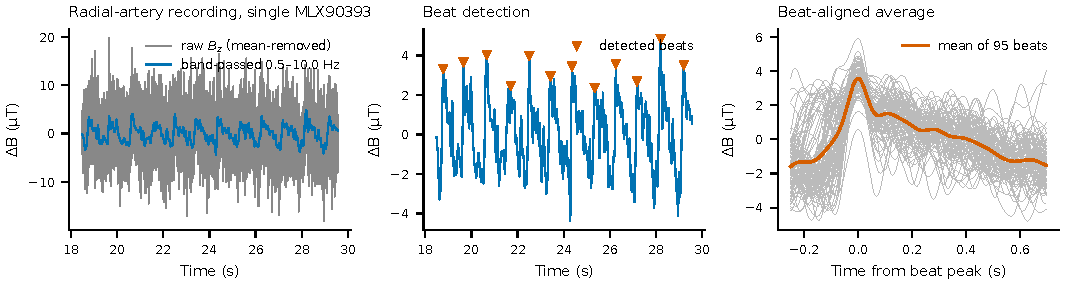
\includegraphics[width=\textwidth]{fig5d_pulse_demo.pdf}
\caption*{\textbf{Preliminary Fig.~5d candidate $\vert$ Pulse micro-vibration
demonstration (real data, single MLX90393, L8/d0.8 cilia, 500~Hz).}
Left: raw and band-passed (0.5--10~Hz) $B_z$ at the radial artery.
Middle: beat detection on the band-passed trace. Right: beat-aligned
individual beats (grey) and their mean ($n=95$ beats, peak
$\approx$3.6~$\mu$T), showing a coherent systolic waveform with a secondary
shoulder. Qualitative demonstration only: no synchronized ECG exists for this
recording, so no heart-rate accuracy or timing claim is made
(notes/pulse\_data\_verdict.md).}
\end{figure}

\begin{figure}[h]
\centering
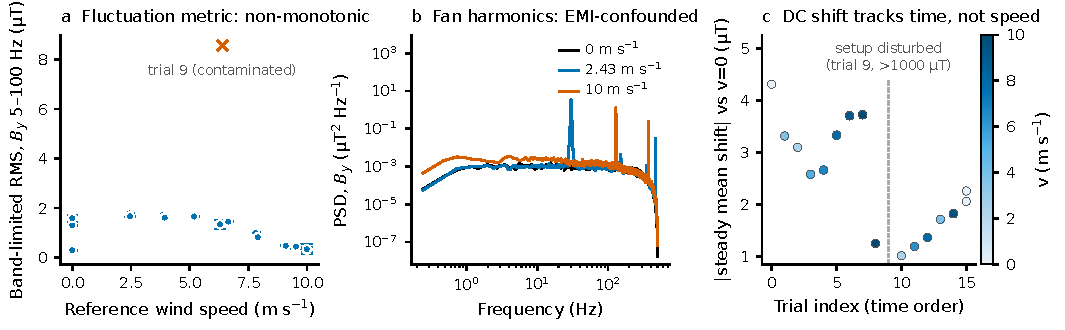
\includegraphics[width=\textwidth]{edx_wind_preliminary.pdf}
\caption*{\textbf{Preliminary airflow data $\vert$ Why the 2025-07-17 session
cannot yield a $\Delta B$--$v$ calibration.} \textbf{(a)}~Band-limited RMS is
non-monotonic in speed. \textbf{(b)}~The response concentrates in narrowband
peaks at fan-rotation harmonics, indistinguishable from fan-motor magnetic
pickup without a bare-sensor control; the broadband floor is
speed-independent. \textbf{(c)}~The steady DC shift follows trial order
(drift and a setup discontinuity at trial~9), not wind speed. Re-measurement
SOP: notes/acquisition\_SOPs.md, SOP-4.}
\end{figure}

\begin{figure}[h]
\centering
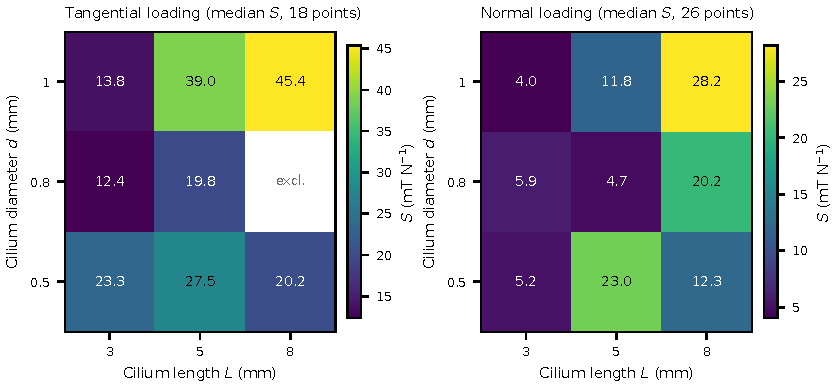
\includegraphics[width=0.85\textwidth]{fig2e_geometry_sensitivity.pdf}
\caption*{\textbf{Preliminary Fig.~2e candidate $\vert$ Geometry-dependent
sensitivity (real data, nine $(L,d)$ combinations, manual loading at
1/2/3~mm depths, ATI force reference).} Median plateau sensitivity
$S=|\Delta B|/F$ per geometry under tangential (left) and normal (right)
loading; per-cell values in mT\,N$^{-1}$. The $(8.0,0.8)$ tangential cell and
one $(8,1.0)$-adjacent artifact point are excluded per QC. The largest median
response occurs for the longest, thickest cilia ($L=8$~mm, $d=1.0$~mm).
Manual-loading depth variability (CV 13.4\%) limits absolute calibration; the
robot-controlled campaign (SOP-1) supersedes these values for force claims.}
\end{figure}

\begin{figure}[h]
\centering
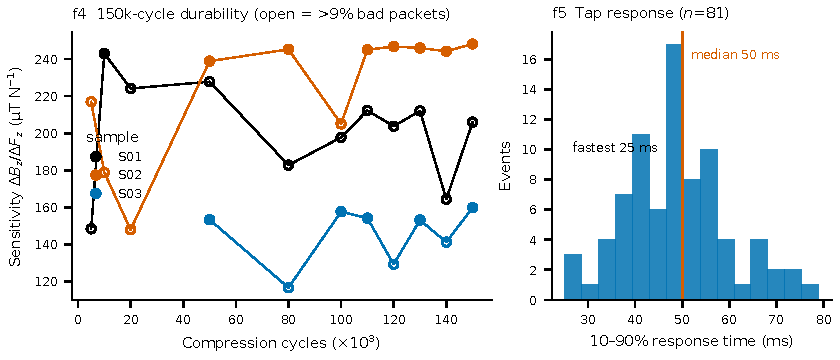
\includegraphics[width=0.85\textwidth]{fig2f_dynamics_durability.pdf}
\caption*{\textbf{Preliminary Fig.~2f candidate $\vert$ Durability and
dynamic response (real data).} \textbf{(a)}~Checkpoint sensitivity
$\Delta B_z/\Delta F_z$ over 150{,}000 compression cycles for three
independent samples; open symbols mark checkpoints with $>$9\% corrupted
acquisition packets (low confidence). Reliable checkpoints show no
significant degradation (within $\pm$4\% from 50k to 150k cycles).
\textbf{(b)}~Distribution of 10--90\% response times across 81 tap events
(fastest 25~ms, median 50~ms).}
\end{figure}

\begin{figure}[h]
\centering
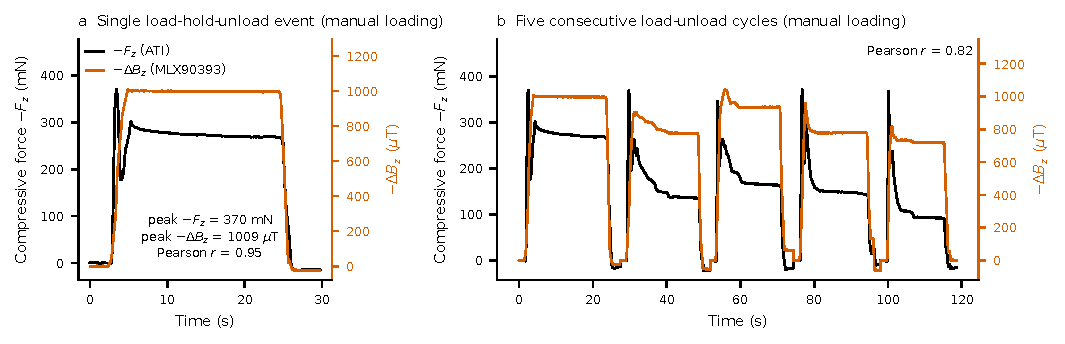
\includegraphics[width=0.9\textwidth]{fig3c_event_alignment.pdf}
\caption*{\textbf{Preliminary Fig.~3 material $\vert$ Force--magnetic
correspondence (real data, manual loading, ATI reference).}
\textbf{(a)}~Single load--hold--unload event: compressive force $-F_z$ and
magnetic response $-\Delta B_z$ (sign conventions on axes), peak 370~mN
$\leftrightarrow$ 1009~$\mu$T, Pearson $r=0.95$. \textbf{(b)}~Five
consecutive cycles, $r=0.82$; amplitude variation reflects manual depth
variability.}
\end{figure}

\begin{figure}[h]
\centering
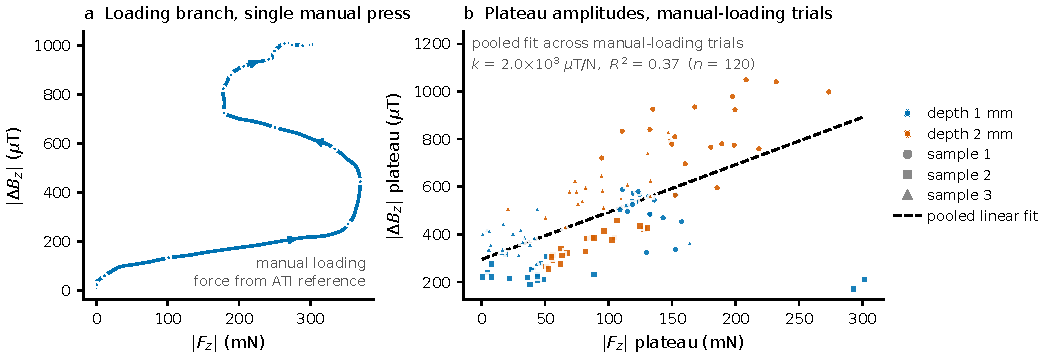
\includegraphics[width=0.9\textwidth]{fig3c_BF_calibration.pdf}
\caption*{\textbf{Preliminary Fig.~3 material $\vert$ $\Delta B$--$F$
relation (real data, manual loading).} \textbf{(a)}~Loading-branch
trajectory of a single press (force relaxation gives the non-monotonic
path). \textbf{(b)}~Plateau amplitudes across 120 manual trials (3 samples
$\times$ 2 target depths): pooled linear fit $k=2.0\times10^3$~$\mu$T/N,
$R^2=0.37$ --- the modest $R^2$ reflects manual depth variability and is
expected to improve substantially under the robot-controlled protocol
(SOP-1).}
\end{figure}

\begin{figure}[h]
\centering
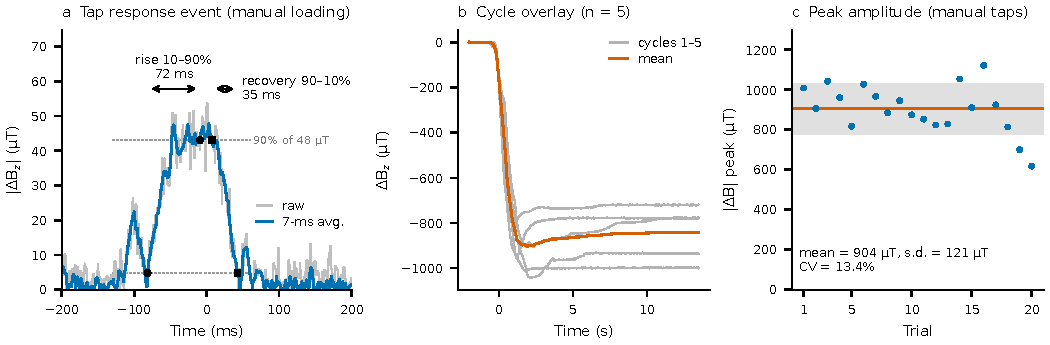
\includegraphics[width=0.9\textwidth]{fig2f_response_event.pdf}
\caption*{\textbf{Preliminary Fig.~2f material $\vert$ Dynamic response and
repeatability (real data).} \textbf{(a)}~Representative median-amplitude tap
event (high-rate acquisition): 10--90\% rise 72~ms, 90--10\% recovery 35~ms
(7-ms moving average; values are smoothing-dependent within $\sim$30--80~ms;
the fastest of 81 events is 25~ms). \textbf{(b)}~Five aligned manual cycles
and mean. \textbf{(c)}~Peak amplitudes across 20 manual trials, CV~13.4\%.}
\end{figure}

\begin{figure}[h]
\centering
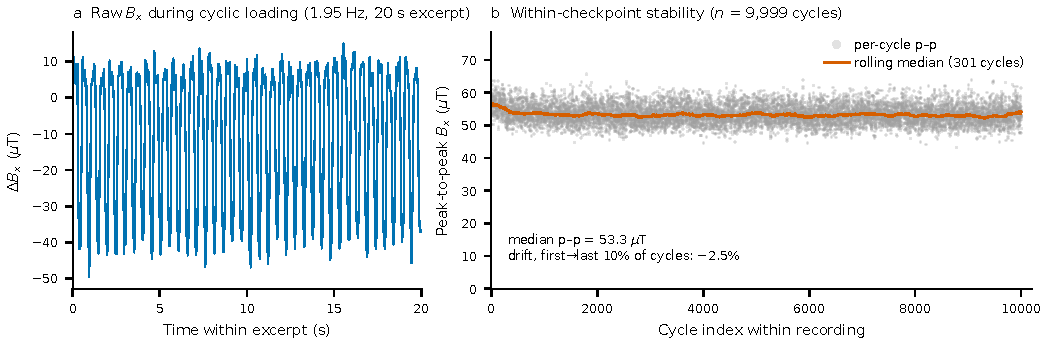
\includegraphics[width=0.9\textwidth]{fig2f_cyclic_stability.pdf}
\caption*{\textbf{Preliminary Fig.~2f material $\vert$ Within-checkpoint
cyclic stability of a $5\times5$ cilia array (real data).}
\textbf{(a)}~Baseline-subtracted $B_x$ during machine-cycled loading
(period 0.512~s, 1.95~Hz; 20-s excerpt) at the 10{,}000-cycle checkpoint.
\textbf{(b)}~Per-cycle peak-to-peak amplitude across all 9{,}999 recorded
cycles: median 53.3~$\mu$T, drift between first and last 10\% of cycles
$-2.5$\%.}
\end{figure}

\begin{figure}[h]
\centering
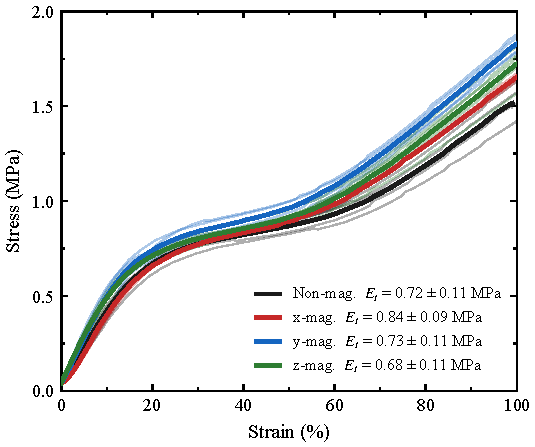
\includegraphics[width=0.62\textwidth]{fig2d_stress_strain_direction.pdf}
\caption*{\textbf{Fig.~2d candidate $\vert$ Stress--strain by magnetization
direction (real data, DIN~EN~ISO~527-1).} Engineering stress (load divided by
each specimen's cross-section $A_0$) versus strain, shown to 100\% strain.
Thin lines: individual specimens; bold lines: group means (averaged only
where all group specimens have data). $E_t$ = linear-fit slope over the
20--40\% strain interval (dimensionless strain), mean\,$\pm$\,s.d.\ from the
machine summary: non-mag.\ $0.72\pm0.11$, $x$ $0.84\pm0.09$, $y$
$0.73\pm0.11$, $z$ $0.68\pm0.11$~MPa. The $x$-magnetized group (aligned with
the tensile axis) shows a trend towards higher stiffness (2 valid
specimens---trend only, no significance claim).}
\end{figure}

\begin{figure}[h]
\centering
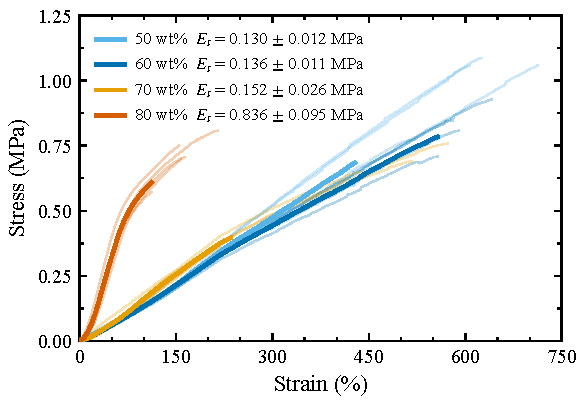
\includegraphics[width=0.62\textwidth]{fig2d_stress_strain_wtpct.pdf}
\caption*{\textbf{Fig.~2a/2d candidate $\vert$ Composition series:
Ecoflex~00-30 with 50--80~wt\% NdFeB (real data).} Full curves to specimen
break. 50--70~wt\% remain compliant ($E_t$ $0.130$--$0.152$~MPa) with
elongation above 400\%; 80~wt\% stiffens roughly sixfold
($0.836\pm0.095$~MPa) with elongation reduced to $\approx$150\%,
defining the compliance--magnetic-loading trade-off for cilia design. Note:
the tester export's per-specimen channel is already stress (kPa), verified
against the summary sheet.}
\end{figure}

\begin{figure}[h]
\centering
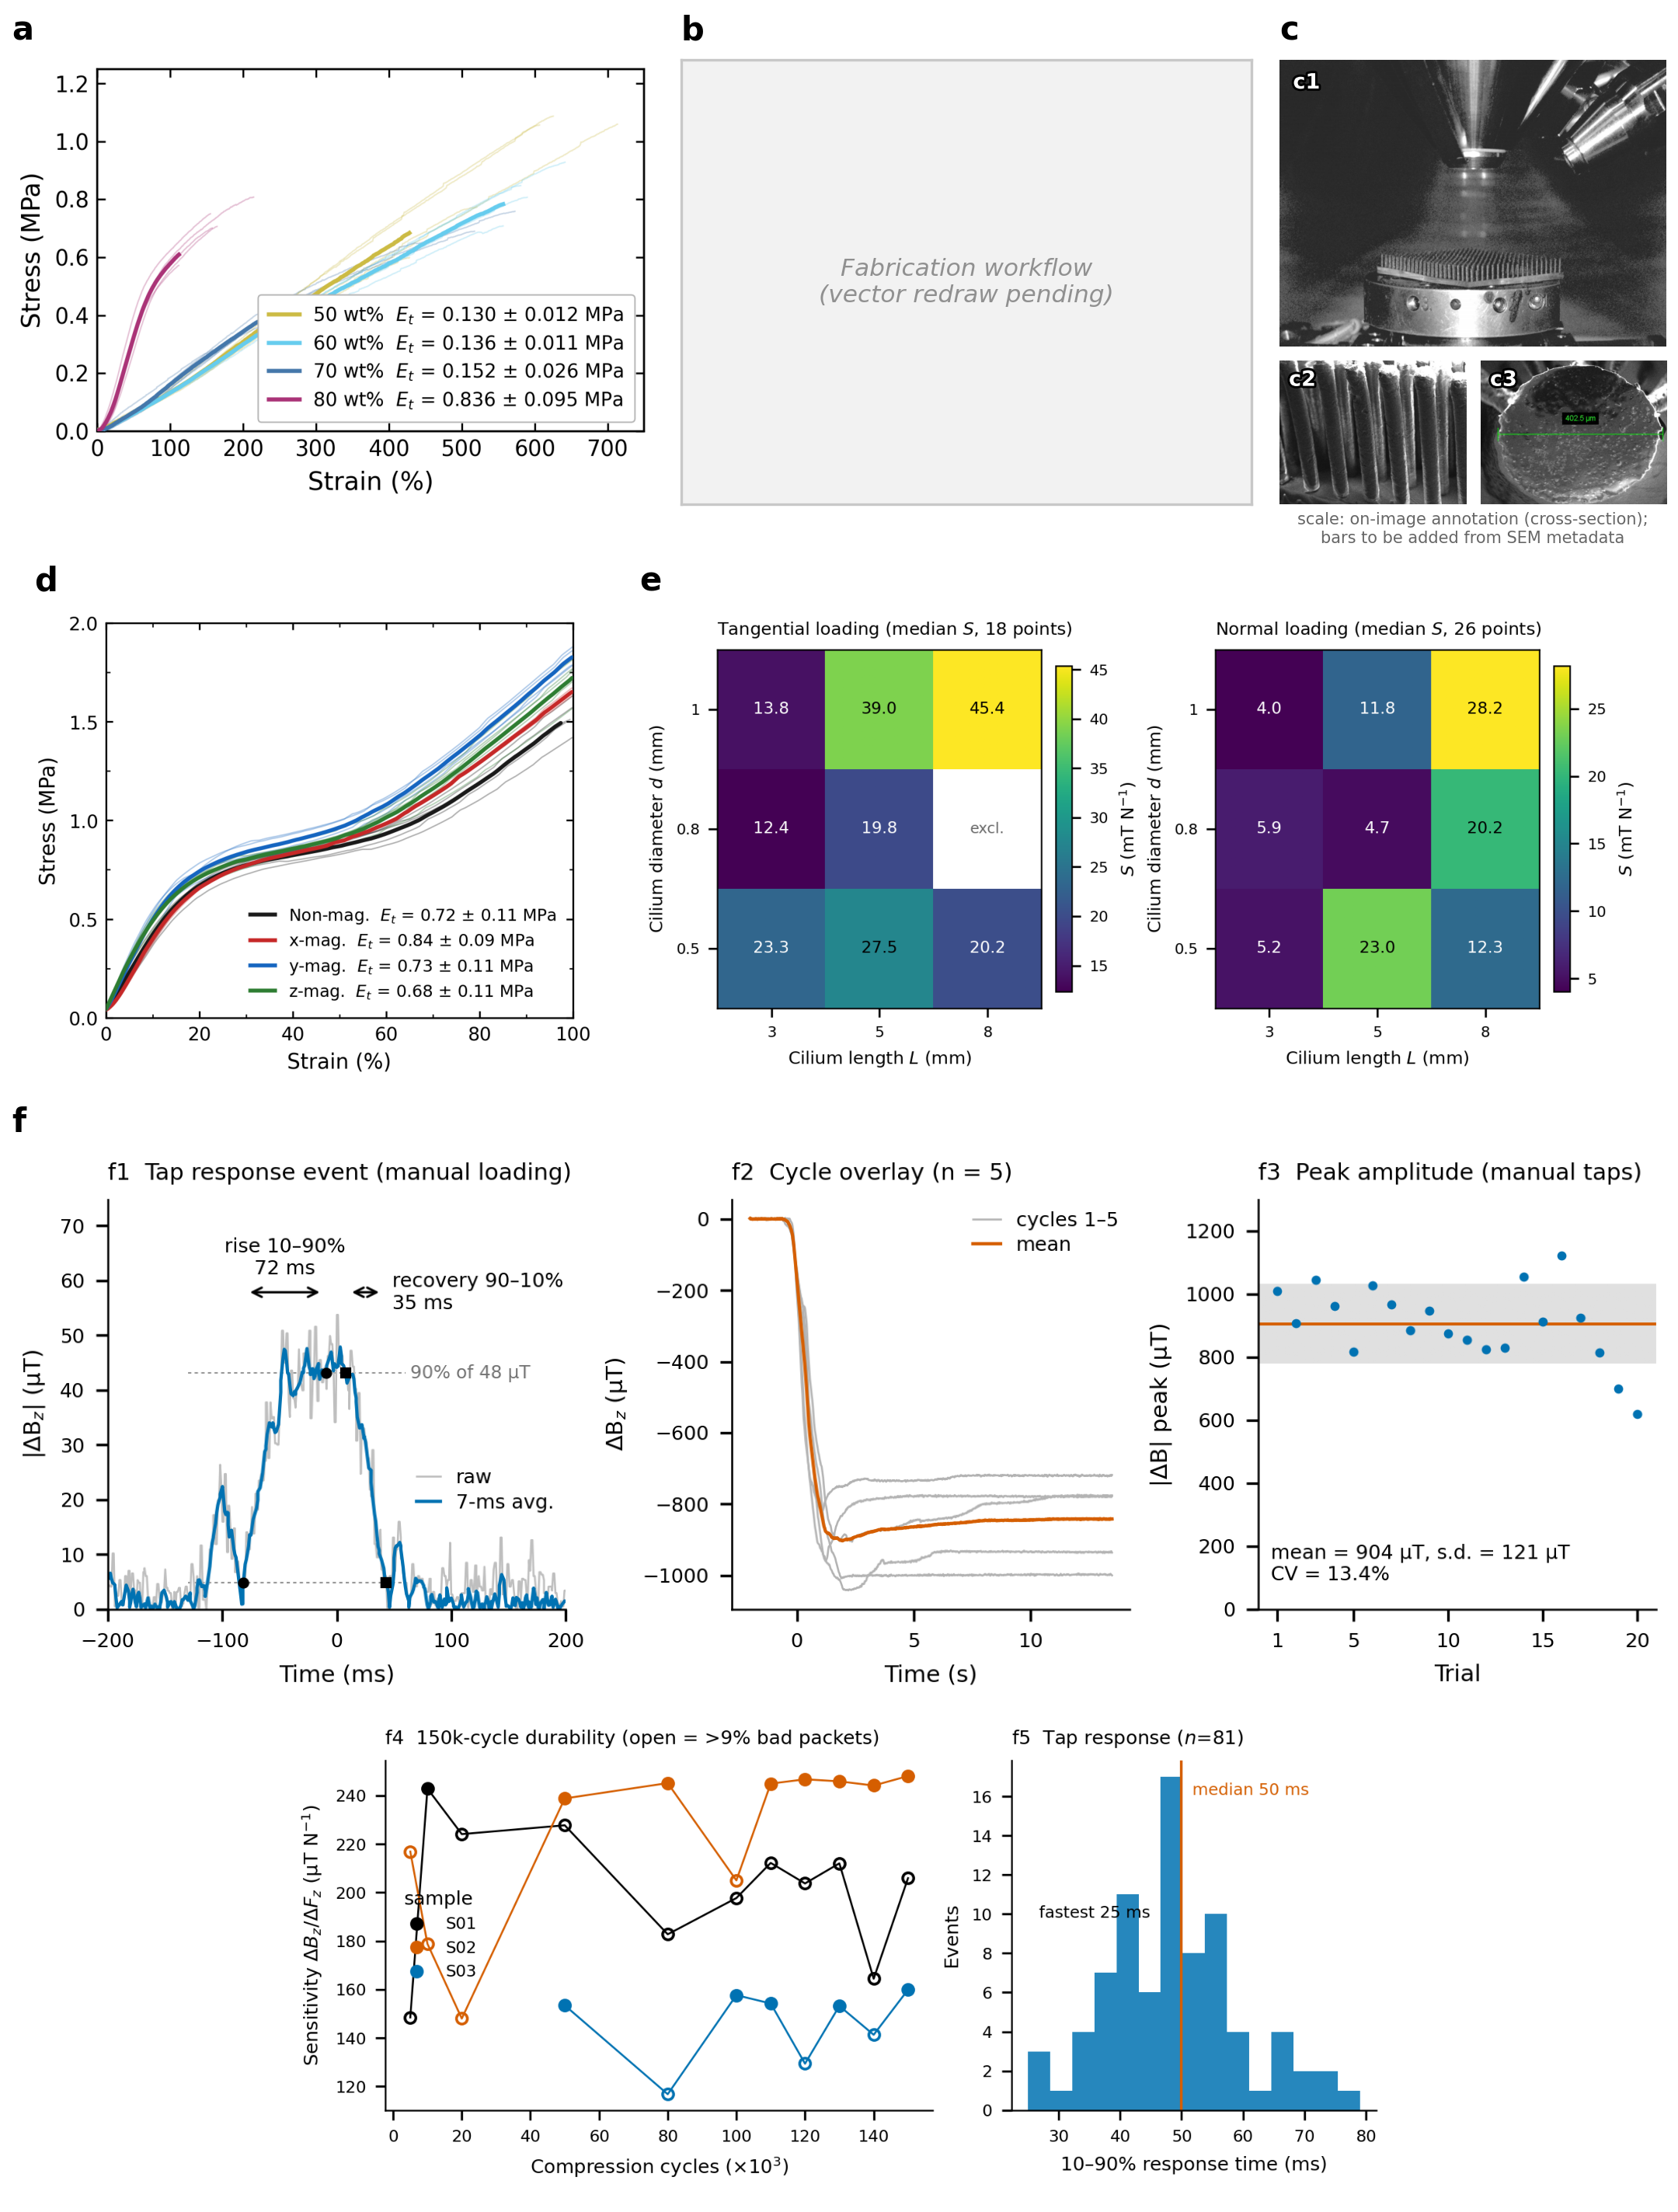
\includegraphics[width=0.95\textwidth]{fig2_composite.png}
\caption*{\textbf{Figure 2 assembly draft (raster; vector originals ship
separately).} \textbf{(a)}~Composition series (Ecoflex~00-30, 50--80~wt\%
NdFeB). \textbf{(b)}~Fabrication workflow (team schematic; fix ``Vaccum''
$\rightarrow$ Vacuum and ``Demode'' $\rightarrow$ Demould in the vector
redraw). \textbf{(c)}~SEM micrographs with on-image scale bars: c1 array
overview (400~$\mu$m), c2 cilia close-up (300~$\mu$m), c3 single-cilium
cross-section (100~$\mu$m bar; measured width 402.5~$\mu$m for nominal
$d=0.5$~mm). \textbf{(d)}~Stress--strain by magnetization
direction. \textbf{(e)}~Geometry--sensitivity heatmaps. \textbf{(f)}~Dynamic
response, repeatability and 150k-cycle durability (sub-panels f1--f5).}
\end{figure}

\begin{figure}[h]
\centering
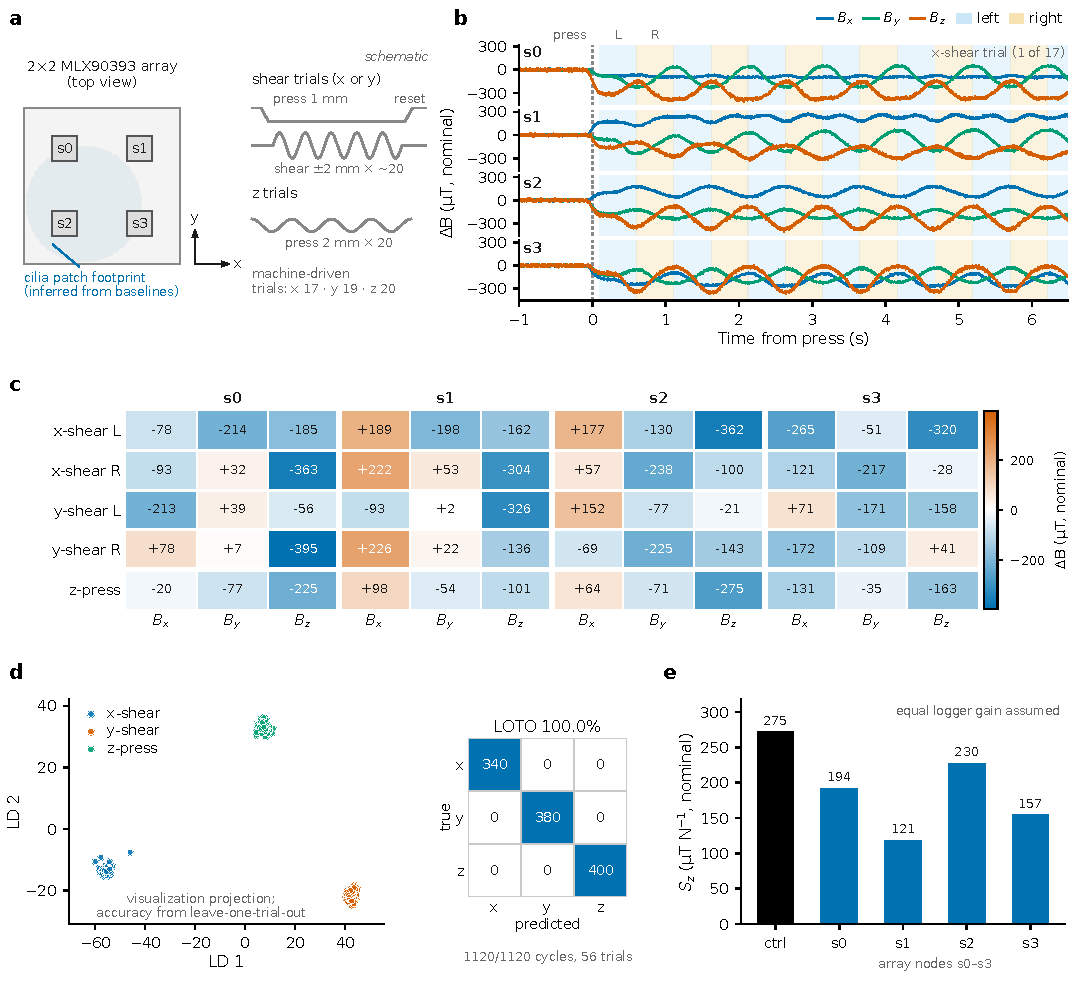
\includegraphics[width=\textwidth]{fig3_quad_main.pdf}
\caption*{\textbf{Fig.~3 candidate (main-figure draft) $\vert$ The local
$2\times2$ tri-axis unit separates loading directions.}
\textbf{(a)}~Schematic: sensor layout (top view; cilia patch footprint
inferred from no-load baselines) and machine-driven protocols (shear trials:
1~mm press then $\pm$2~mm shear $\times\sim$20; $z$ trials: 2~mm press
$\times$20; usable trials $x$ 17 of 20, $y$ 19 of 21, $z$ 20 of 20 after
alignment quality control). \textbf{(b)}~Representative $x$-shear trial:
baseline-subtracted 12-channel response (four sensors $\times$
$B_x,B_y,B_z$), left/right shear stages shaded; the four sensors respond
with distinct, spatially differential signatures. \textbf{(c)}~Fingerprint
matrix: trial-averaged stage response per channel for the five loading
conditions (nominal logger $\mu$T). \textbf{(d)}~Per-cycle 12-channel
samples in the LDA plane (visualization projection) and leave-one-trial-out
confusion matrix: 100.0\% (1120/1120 cycles, 56 trials; shuffled-label
control at chance). Two caveats: features are built from protocol stage
labels (shear cycles as right$-$left differentials, $z$ as press-plateau
means), so this is class separability rather than blind real-time decoding;
and each class was acquired as a contiguous same-day block, so
trial-held-out validation cannot fully exclude block-level drift as a cue.
\textbf{(e)}~$z$-press sensitivity of an isolated single sensor (ctrl)
versus the four array nodes; the spread reflects patch--sensor offset
geometry (equal logger gain assumed). Force amplitude is not decodable under
this displacement-controlled protocol ($|r|\leq0.23$; see analysis notes)
--- force decoding awaits the force-controlled xArm campaign.}
\end{figure}

\paragraph{Supplementary Videos.}
(1) $2\times2$ inverse decoding; (2) bubble touch; (3) 44-node real-time map;
(4) no-contact artifact test; (5) wind-tunnel pose change;
(6) ECG-synchronized pulse.


\end{document}
